%% ============================================================
%%  Connector OS — Infrastructure for Governed AI
%%  A Brief for Greylock Partners
%%  GlobalSushrut, Inc. — 2026
%% ============================================================
\documentclass[11pt,a4paper]{article}

\usepackage[T1]{fontenc}
\usepackage[utf8]{inputenc}
\usepackage{lmodern}
\usepackage{microtype}
\usepackage[top=1.0in,bottom=1.0in,left=1.15in,right=1.15in]{geometry}
\usepackage[dvipsnames,table]{xcolor}
\usepackage{graphicx}
\usepackage{enumitem}
\usepackage{setspace}
\usepackage{array,tabularx,booktabs,longtable}
\usepackage{caption}
\usepackage[most]{tcolorbox}
\usepackage{fancyhdr}
\usepackage{titlesec}
\usepackage{fontawesome5}
\usepackage{tikz}
\usetikzlibrary{arrows.meta,positioning,calc,shapes.geometric,fit}
\usepackage[
  colorlinks=true,
  linkcolor=MidnightBlue,
  urlcolor=MidnightBlue,
  citecolor=MidnightBlue,
  pdftitle={Connector OS -- Infrastructure for Governed AI -- Greylock Brief},
  pdfauthor={GlobalSushrut Inc.},
]{hyperref}

%% ── Palette ──────────────────────────────────────────────────
\definecolor{CBlue}{RGB}{24,78,160}
\definecolor{CGreen}{RGB}{0,130,90}
\definecolor{CAmber}{RGB}{175,115,0}
\definecolor{CRed}{RGB}{176,30,30}
\definecolor{CNavy}{RGB}{15,23,42}
\definecolor{CGray}{RGB}{100,116,139}
\definecolor{CSoft}{RGB}{246,248,252}
\definecolor{CGreylock}{RGB}{32,58,114}

%% ── tcolorbox styles ─────────────────────────────────────────
\tcbset{base/.style={breakable,enhanced,arc=4pt,boxrule=0.7pt,
  fonttitle=\bfseries\small,top=6pt,bottom=6pt,left=8pt,right=8pt}}

\newtcolorbox{keybox}[1]{base,title={#1},
  colback=CBlue!5,colframe=CBlue!65,coltitle=white,
  attach boxed title to top left={yshift=-2mm,xshift=5mm},
  boxed title style={colback=CBlue,arc=2pt,boxrule=0pt}}

\newtcolorbox{greybox}[1]{base,title={#1},
  colback=CGreylock!5,colframe=CGreylock!70,coltitle=white,
  attach boxed title to top left={yshift=-2mm,xshift=5mm},
  boxed title style={colback=CGreylock,arc=2pt,boxrule=0pt}}

\newtcolorbox{insightbox}[1]{base,title={#1},
  colback=CGreen!5,colframe=CGreen!65,coltitle=white,
  attach boxed title to top left={yshift=-2mm,xshift=5mm},
  boxed title style={colback=CGreen,arc=2pt,boxrule=0pt}}

\newtcolorbox{warnbox}[1]{base,title={#1},
  colback=CAmber!7,colframe=CAmber!75,coltitle=white,
  attach boxed title to top left={yshift=-2mm,xshift=5mm},
  boxed title style={colback=CAmber,arc=2pt,boxrule=0pt}}

\newtcolorbox{dangerbox}[1]{base,title={#1},
  colback=CRed!5,colframe=CRed!65,coltitle=white,
  attach boxed title to top left={yshift=-2mm,xshift=5mm},
  boxed title style={colback=CRed,arc=2pt,boxrule=0pt}}

%% ── Typography ───────────────────────────────────────────────
\setstretch{1.10}
\setlist[itemize]{itemsep=3pt,topsep=3pt}
\setlist[enumerate]{itemsep=3pt,topsep=3pt}
\captionsetup{labelfont=bf,skip=5pt,font=small}

\titleformat{\section}
  {\normalfont\Large\bfseries\color{CBlue}}{\thesection}{0.8em}{}[\vspace{-4pt}\textcolor{CBlue!30}{\rule{\linewidth}{0.5pt}}]
\titleformat{\subsection}
  {\normalfont\large\bfseries\color{CBlue!80}}{\thesubsection}{0.7em}{}
\titleformat{\subsubsection}
  {\normalfont\normalsize\bfseries\color{CGray}}{\thesubsubsection}{0.6em}{}
\titlespacing*{\section}{0pt}{16pt}{6pt}
\titlespacing*{\subsection}{0pt}{10pt}{4pt}

%% ── Header / Footer ──────────────────────────────────────────
\pagestyle{fancy}\fancyhf{}
\fancyhead[L]{\small\color{CGray}\textsc{Connector OS}}
\fancyhead[R]{\small\color{CGray}Infrastructure for Governed AI}
\fancyfoot[C]{\small\color{CGray}\thepage}
\renewcommand{\headrulewidth}{0.4pt}

%% ── Convenience macros ───────────────────────────────────────
\newcommand{\connector}{\textbf{Connector OS}}
\newcommand{\greylock}{\textbf{Greylock}}

%% ============================================================
\begin{document}
\setlength{\parindent}{0pt}
\setlength{\parskip}{6pt}

%% ── TITLE PAGE ───────────────────────────────────────────────
\begin{titlepage}
\pagecolor{CNavy}\color{white}
\vspace*{1.8cm}
\begin{center}
  {\fontsize{10}{12}\selectfont\scshape\color{white!60} Confidential — For Discussion}\\[0.9cm]
  {\fontsize{42}{50}\selectfont\bfseries Connector OS}\\[0.3cm]
  {\fontsize{18}{22}\selectfont\color{white!85} Infrastructure for Governed AI}\\[1.4cm]
  \textcolor{white!25}{\rule{0.65\textwidth}{0.5pt}}\\[1.4cm]
  \begin{minipage}{0.82\textwidth}\centering
    \colorbox{white!10}{%
      \parbox{0.9\textwidth}{\centering\large\color{white}
        Your AI agents are running naked across your infrastructure.\\[8pt]
        They spend your money, touch your customer data, and make\\
        decisions you cannot prove or audit.\\[12pt]
        \textbf{Connector OS is the execution control layer that fixes this.}
      }
    }
  \end{minipage}\\[1.8cm]
  {\large\color{white!75} A Brief for Greylock Partners}\\[0.3cm]
  {\normalsize\color{white!55} GlobalSushrut, Inc. \enspace\textbullet\enspace 2026}
\end{center}
\vfill
\noindent\textcolor{white!20}{\rule{\textwidth}{0.4pt}}\\[4pt]
{\footnotesize\color{white!50}
  This document answers the questions raised by our buyer one-pager and positions Connector OS
  as infrastructure, not a product feature. It is written with Greylock's stated investment
  thesis in mind: \emph{Visibility, Governance, and Auditability} for AI — the same
  three pillars that define Connector's architecture.
}
\end{titlepage}
\nopagecolor\color{black}

%% ── TABLE OF CONTENTS ────────────────────────────────────────
\tableofcontents
\clearpage

%% ============================================================
\section{The Greylock Lens: Why This Brief Is Written This Way}
\label{sec:greylock-lens}

Greylock has publicly articulated the most precise framing of the AI security problem we have seen from any investor. Jason Risch and Saam Motamedi wrote in \emph{Securing AI}:

\begin{greybox}{Greylock — Securing AI (verbatim)}
\emph{``The immediate priority CISOs face is \textbf{visibility, governance, and auditability} to mitigate risk\ldots
AI represents a new and currently unsecured surface area (much as cloud did in a previous platform shift)\ldots
As AI agents enter the enterprise, interact with systems, and are potentially granted permissions to modify state,
they become a \textbf{new identity surface area} to govern.''}
\end{greybox}

Those three words — Visibility, Governance, Auditability — are the exact three structural properties that Connector OS
produces for every agent execution. This is not a coincidence of language. Greylock has identified the same structural gap that Connector's architecture is designed to close.

\subsection{What Greylock Has Learned from Cloud Security}

The Greylock thesis draws an explicit parallel between AI security today and cloud security in 2012--2015:

\begin{itemize}
  \item The infrastructure layers need to stabilize before the right durable architecture emerges.
  \item Many of the largest cloud security companies launched \emph{years after} the cloud migration began — because enterprises only face the security problem when they are already deep in production.
  \item The first durable products solve posture (CSPM) and runtime (D\&R) — in that order.
\end{itemize}

Enterprises are already deep in AI production in 2026. They have already deployed agents. The posture problem has landed. The runtime problem is here now. \connector\ is the runtime control plane.

\subsection{What Greylock Specifically Calls Out as Missing}

From the same Greylock research, the five unsolved gaps are:

\begin{center}
\begin{tabular}{@{}p{0.35\linewidth}p{0.58\linewidth}@{}}
\toprule
\textbf{Gap Greylock Identified} & \textbf{Connector OS Structural Answer} \\
\midrule
Prompt \& response audit logs & Chain 1 (HMAC Audit Chain) — every input/output tamper-evident \\
PII leaking into LLM context & Chain 9 (Isolation Chain) + namespace firewall — structurally blocked \\
Agent identity as new surface & Agent DID + namespace isolation + CCL contract capability declarations \\
Non-determinism / unpredictability & CCL contracts compile policy; Chain 3 (Dehallucination) grounds every output \\
Runtime detection \& response & Policy engine + HITL gate + governance chain — blocks in real time \\
\bottomrule
\end{tabular}
\end{center}

\clearpage

%% ============================================================
\section{The Problem: Three Structural Gaps in Every AI Deployment}
\label{sec:problem}

Every enterprise deploying AI agents in production faces three structural gaps that no current tool closes.

\subsection{Gap 1 — Silent Budget Drain}

\begin{dangerbox}{The Failure Mode}
An agent enters a retry loop at 3 AM. No human is watching. By morning, \$18{,}000 in
LLM API spend has been consumed on a single broken workflow. Nobody knew. Nobody could have known.
\end{dangerbox}

The root cause is architectural: AI agents have no native concept of budget. The LLM provider charges per token.
The orchestration framework passes requests through. There is no layer between the agent and the provider that
enforces a spending limit, counts tokens in real time, and terminates the agent when the budget is exhausted.

\textbf{Current workarounds that don't work:}
\begin{itemize}
  \item Cloud billing alerts fire 24--48 hours after the fact, by which point the damage is done.
  \item Application-level counters break under retries, multi-agent delegation, and parallel execution.
  \item LLM providers offer no per-agent, per-workflow budget enforcement — only account-level limits.
\end{itemize}

\textbf{What Connector does:} The gateway service intercepts every LLM call. Token counts are computed from
the provider's actual response. A per-agent cost ledger is updated in real time. CCL contracts declare a
\texttt{budget.tokens} ceiling. If the ceiling is hit, the contract terminates — not the application, the
\emph{contract} — with a signed receipt proving why it stopped.

\subsection{Gap 2 — The Compliance Nightmare}

\begin{dangerbox}{The Failure Mode}
A healthcare AI agent reads a patient chart to generate a care recommendation. The agent's context window
now contains PHI. That context is sent to the LLM provider. You have just violated HIPAA §164.502(b)
minimum necessary and §164.312(a) access controls — with no proof that you prevented it or that it happened.
\end{dangerbox}

\textbf{Why regulations are structurally violated by default:}
\begin{itemize}
  \item LLM context construction is opaque — developers do not inspect what the agent injected.
  \item Orchestration frameworks (LangChain, CrewAI, AutoGen) have no data classification layer.
  \item Compliance is enforced by policy documents, not by the runtime system.
\end{itemize}

\textbf{What Connector does:} The namespace firewall classifies data at the storage layer.
PHI lives in \texttt{/p/} namespace with \texttt{SecurityLevel::Restricted}. The selective context engine
strips or pseudonymizes \texttt{/p/} content before it reaches the LLM. Chain 9 (Isolation Chain) records
every access attempt — authorized and unauthorized — in a tamper-evident log. A single API call produces
a cryptographic proof bundle covering HIPAA, SOC 2 (all five TSC), GDPR, and EU AI Act simultaneously.

\subsection{Gap 3 — Blind Trust Is Not a Strategy}

\begin{dangerbox}{The Failure Mode}
An agent sends an email to a customer. Later, a complaint arrives. Your team asks: what data did
the agent use? What decision did it make? Who approved it? The answer is: nobody knows. There is no
record. There is no proof. There is nothing to show a regulator, a customer, or a board.
\end{dangerbox}

\textbf{Why auditability is structurally absent:}
\begin{itemize}
  \item LLM providers log tokens, not decisions.
  \item Application logs record API calls, not governance events.
  \item No current tool produces a cryptographic, third-party-verifiable proof of what an AI agent decided and why.
\end{itemize}

\textbf{What Connector does:} Every agent execution produces signed, cryptographically-linked receipts
across 9 independent chains. The proof bundle is verifiable without access to a live Connector node.
A third party — an auditor, a regulator, a court — can verify the bundle using only SHA-256 and Ed25519,
the same primitives used to verify Bitcoin transactions.

\clearpage

%% ============================================================
\section{The Architecture: How Connector OS Works}
\label{sec:architecture}

Connector OS is not middleware that wraps LLM calls. It is a control plane that sits between AI agents
and the systems they act on — enforcing policy, recording evidence, and producing cryptographic proof.

\subsection{The Three-Stage Pipeline}

\begin{center}
\begin{tikzpicture}[
  node distance=0.5cm,
  box/.style={draw=CBlue!50,fill=CBlue!5,rounded corners=6pt,
              minimum height=1.8cm,minimum width=3.6cm,align=center,font=\bfseries\small},
  arrow/.style={-{Stealth[length=8pt]},CBlue!60,line width=2pt},
  label/.style={font=\footnotesize\color{CGray},align=center}
]
\node[box] (I) {\faLock\\[4pt] ISOLATE\\{\normalfont\footnotesize\color{CGray} Agent Vaults}};
\node[box,right=1.4cm of I] (G) {\faSlidersH\\[4pt] GOVERN\\{\normalfont\footnotesize\color{CGray} Policy + Budget + HITL}};
\node[box,right=1.4cm of G] (V) {\faCheckDouble\\[4pt] VERIFY\\{\normalfont\footnotesize\color{CGray} Cryptographic Proof}};
\draw[arrow] (I) -- (G);
\draw[arrow] (G) -- (V);

\node[label,below=0.4cm of I] {Separate execution\\per agent.\\ Knowledge never blends.};
\node[label,below=0.4cm of G] {Nothing runs outside\\your defined rules.\\Budget enforced at runtime.};
\node[label,below=0.4cm of V] {Signed receipt for\\every decision.\\ Full audit trail.};
\end{tikzpicture}
\end{center}

\subsubsection{Stage 1 — Isolate (Agent Vaults)}
Each agent runs inside a typed namespace sandbox. Its memory, knowledge, tools, and instructions
are bound to its namespace. Agents cannot read each other's data. PHI namespaces (\texttt{/p/}) cannot
be included in LLM context without a declared capability in the agent's compiled CCL contract.
Cross-agent data flow requires an explicit, audited handoff — not a function call.

\subsubsection{Stage 2 — Govern (The Safety Net)}
The governance pipeline enforces three independent gates before any agent action executes:

\begin{enumerate}
  \item \textbf{Policy Check} — CCL contract declares allowed/denied tools, states, and transitions.
        The policy engine (Cedar-compatible, deny-overrides) blocks anything undeclared.
  \item \textbf{Budget Check} — Real token count against the contract's \texttt{budget.tokens} ceiling.
        If exceeded, the contract terminates with a signed receipt — not a crash.
  \item \textbf{HITL Gate} — Confidence thresholds declared in the CCL contract trigger human-in-the-loop
        review for high-stakes actions. The approver's identity and decision are recorded in the Compliance Chain.
\end{enumerate}

\subsubsection{Stage 3 — Verify (The Proof Plane)}
Every governed execution produces entries across 9 independent cryptographic chains:

\begin{center}
\small
\begin{tabular}{@{}llp{0.48\linewidth}@{}}
\toprule
\textbf{Chain} & \textbf{Name} & \textbf{What it records} \\
\midrule
1 & Audit Chain & Every system event — HMAC-SHA256 linked \\
2 & Memory Chain & Every namespace write — CID-linked per namespace \\
3 & Dehallucination & Every LLM output linked to grounding memory packets \\
4 & Compliance & Every governance decision tagged with regulation IDs \\
5 & Governance & Every CCL contract step executed \\
6 & Execution & Every tool call receipt — content addressed \\
7 & Trust & Per-agent reputation score history \\
8 & Proof & Root attestation tree anchoring all chains \\
9 & Isolation & Every namespace access — authorized and unauthorized \\
\bottomrule
\end{tabular}
\end{center}

A single API call — \texttt{POST /api/v1/proof/generate} — traverses all 9 chains and returns
a JSON proof bundle signed with the node's Ed25519 keypair. The bundle is
\textbf{verifiable without access to a live Connector node}. This is the property that makes
Connector evidence usable in regulatory proceedings.

\subsection{CCL Contracts — Policy as Compiled Code}

CCL (Connector Contract Language) is a domain-specific language that compiles agent behavior into a
\emph{SolutionContract} — a content-addressed, Ed25519-signed, machine-executable governance unit.

\begin{keybox}{CCL Contract Example — Medical Triage Agent}
\begin{verbatim}
contract patient-triage-agent {
  version: "1.0"
  identity: "triage-v1"
  
  budget {
    tokens:    50000
    cost_usd:  0.80
  }
  
  tools  { allow: [read_ehr, send_alert]  deny: [delete, export_data] }
  memory { read:  [/m/triage/, /k/protocols/]
           write: [/m/triage/]             deny_read: [/p/billing/] }
  
  governance {
    hipaa: true
    hitl_on_confidence_below: 0.75
  }
}
\end{verbatim}
\end{keybox}

The CCL compiler produces a \texttt{cls1-sha256-\ldots} CID — a content address that uniquely identifies
the compiled contract. Any modification produces a different CID — making contract tampering detectable.

\clearpage

%% ============================================================
\section{Infrastructure Positioning — Crystal Clear}
\label{sec:positioning}

\begin{insightbox}{The One-Sentence Positioning}
\large\centering
Connector OS is to AI agents what a Linux kernel is to processes — the mandatory substrate
through which all resource access, policy enforcement, and audit recording flows.
\end{insightbox}

\subsection{What Connector IS — and What It Is NOT}

\begin{center}
\begin{tabular}{@{}p{0.46\linewidth}p{0.46\linewidth}@{}}
\toprule
\textbf{\textcolor{CGreen}{\faCheckCircle}\enspace Connector IS} & \textbf{\textcolor{CRed}{\faTimesCircle}\enspace Connector IS NOT} \\
\midrule
An execution control plane for AI agents & An AI model or foundation model \\
A policy enforcement runtime & An orchestration framework (LangChain, CrewAI) \\
A cryptographic audit and proof layer & A cloud observability tool (Datadog, Grafana) \\
A compliance-structural layer (HIPAA/SOC2/GDPR) & A compliance SaaS with checkboxes \\
An infrastructure primitive (like a kernel) & A wrapper on top of the LLM API \\
Self-hosted, customer-data-sovereign & A cloud-native SaaS requiring data egress \\
Model-agnostic (DeepSeek, GPT-4o, Claude) & Coupled to any specific AI provider \\
\bottomrule
\end{tabular}
\end{center}

\subsection{Where Connector Sits in the Stack}

\begin{center}
\begin{tikzpicture}[
  layer/.style={draw,rounded corners=4pt,minimum width=10cm,minimum height=0.9cm,
                align=center,font=\small\bfseries},
  outside/.style={layer,fill=gray!10,draw=gray!40,text=gray},
  connector/.style={layer,fill=CBlue!12,draw=CBlue,text=CBlue!80!black,
                    minimum height=1.15cm,font=\normalsize\bfseries},
]
\node[outside] (app) {Your Application / Business Logic};
\node[outside,below=0.18cm of app] (orch) {Orchestration Layer (LangChain / CrewAI / Custom)};
\node[connector,below=0.18cm of orch] (conn)
  {\faShieldAlt\enspace CONNECTOR OS — Execution Control Plane \enspace\faShieldAlt\\
   {\small\normalfont\color{CBlue!70} Isolate \textbullet\ Govern \textbullet\ Verify \textbullet\ Audit \textbullet\ Prove}};
\node[outside,below=0.18cm of conn] (llm) {LLM Providers (OpenAI / Anthropic / DeepSeek / Open-Source)};
\node[outside,below=0.18cm of llm] (infra) {Your Infrastructure (Databases / APIs / Cloud Services)};
\end{tikzpicture}
\end{center}

\textbf{Connector sits at the only layer that can simultaneously see:}
the agent's declared intent (CCL contract), the data it is about to touch (namespace), the cost
it is about to incur (token count), and the system it is about to act on (tool call).
No other layer can see all four at once.

\subsection{Why LLM Providers Won't Build This}

OpenAI, Anthropic, and Google provide LLM inference. Their business model is maximizing token throughput.
Building a control plane that blocks, limits, and audits their own API calls is structurally at odds
with their revenue model. They also cannot see the customer's data namespaces, CCL contracts, or
organizational compliance requirements — these live in the customer's environment.

\textbf{Evidence:} OpenAI's ``Usage Limits'' are account-level spending caps set by the customer.
They are not per-agent, not per-workflow, not cryptographically signed, and not regulation-tagged.
They are billing controls, not governance controls.

\subsection{Why Orchestration Frameworks Won't Build This}

LangChain, CrewAI, AutoGen, and similar frameworks provide agent composition primitives.
Their architecture processes requests sequentially and does not include:

\begin{itemize}
  \item A compiler step that verifies policy before execution begins.
  \item A content-addressed proof layer that makes audit records tamper-evident.
  \item A namespace isolation model that classifies data by sensitivity level.
  \item A cryptographic chain that third parties can verify without trusting the framework vendor.
\end{itemize}

These are not features these frameworks are missing — they require a different \emph{architectural layer}
underneath the framework. Connector is that layer. Frameworks run on top of it.

\subsection{Why Cloud Providers Won't Build This}

AWS, Azure, and GCP are infrastructure providers. Their AI governance offerings (AWS Bedrock Guardrails,
Azure AI Content Safety) operate at the model I/O layer — they filter prompts and responses.
They do not:

\begin{itemize}
  \item Enforce per-agent budget ceilings with real-time token counting.
  \item Compile agent behavior into a signed, content-addressed contract.
  \item Produce a regulation-tagged proof bundle covering HIPAA, SOC 2, GDPR, and EU AI Act simultaneously.
  \item Work across multiple cloud providers and self-hosted models in the same governance plane.
\end{itemize}

Multi-cloud and model-agnostic governance is structurally outside what a single cloud provider can deliver.

\clearpage

%% ============================================================
\section{Answering the Buyer One-Pager}
\label{sec:buyer-answers}

The buyer one-pager raises six implicit questions. This section answers each with precision.

\subsubsection*{Q1: What exactly is Connector OS?}

\connector\ is an \textbf{execution control layer for AI agents}. It is a self-hosted runtime that
sits between your AI agents and everything they touch — LLM providers, databases, APIs, and external
services. It enforces policy, records cryptographic evidence, and produces compliance proof bundles
that satisfy HIPAA, SOC 2, GDPR, and the EU AI Act from a single API call.

\subsubsection*{Q2: How does the ``Silent Budget Drain'' get fixed?}

Every LLM call flows through the gateway service. Real token counts from the provider's response
are written to a per-agent cost ledger (SQLite, per-agent key). The CCL contract declares a
\texttt{budget.tokens} ceiling. When the ceiling is hit, the contract state machine moves to
\texttt{budget\_exceeded} — the agent stops, a signed receipt records why, and no further
LLM calls are authorized. This happens in the same request-response cycle as the offending call.

\subsubsection*{Q3: How does the ``Compliance Nightmare'' get fixed structurally?}

Data classification happens at the namespace layer, not the application layer.
PHI is stored in \texttt{/p/} namespaces with \texttt{SecurityLevel::Restricted}.
The selective context engine intercepts context construction: any \texttt{/p/} content is
pseudonymized before the LLM prompt is assembled. Chain 9 records every \texttt{/p/} access.
The proof bundle shows — cryptographically — that PHI was not included in the LLM context.
A regulator does not need to trust your word. They verify the bundle.

\subsubsection*{Q4: What does ``Blind Trust Is Not a Strategy'' mean in practice?}

Without Connector, when an agent makes a wrong decision, your options are: check application logs
(no governance context), ask the LLM provider (they logged tokens, not decisions), or reconstruct
from memory (impossible if the agent session has ended). With Connector, every decision produces
a cross-chain proof entry. You can call \texttt{connectorctl explain <decision-id>} and see:
what data the agent read, which CCL step it was on, what the LLM was given, what it returned,
whether HITL was triggered, and who approved it — all cryptographically linked.

\subsubsection*{Q5: What are the three guarantees (Prevent / Enforce / Prove)?}

\begin{center}
\begin{tabular}{@{}p{0.13\linewidth}p{0.38\linewidth}p{0.40\linewidth}@{}}
\toprule
\textbf{Pillar} & \textbf{Structural mechanism} & \textbf{Evidence produced} \\
\midrule
\textbf{Prevent} & Namespace firewall blocks PHI from reaching LLM context &
  Chain 9 entry: \texttt{phi\_in\_llm\_context: false} \\
\textbf{Enforce} & CCL contract + policy engine + budget gate block every unauthorized action &
  Chain 5 entry: \texttt{contract\_step, policy\_applied} \\
\textbf{Prove} & 9-chain proof bundle signed with Ed25519, verifiable offline &
  \texttt{proof\_root: soe1-sha256-\ldots, verifiable: true} \\
\bottomrule
\end{tabular}
\end{center}

\subsubsection*{Q6: What does the 30-day pilot produce?}

One workflow. Full governance. At the end of 30 days, the pilot customer receives:

\begin{itemize}
  \item A per-agent cost ledger showing exact LLM spend with provider-verified token counts.
  \item A regulation-tagged compliance export covering every framework they declared in CCL contracts.
  \item A chain integrity report showing all 9 chains intact with zero tampered entries.
  \item A signed proof bundle for each agent run — verifiable without Connector by any auditor.
\end{itemize}

This is not a demo. This is production evidence. It is what the customer takes to their compliance
officer, their board, and their regulator.

\clearpage

%% ============================================================
\section{Moat and Defensibility}
\label{sec:moat}

\begin{warnbox}{The Core Defensibility Claim}
Once a regulated enterprise generates compliance proof bundles from Connector, they cannot
remove Connector without destroying their audit trail. The moat is compliance lock-in —
the same lock-in that made Okta irreplaceable for identity and Palo Alto Networks
irreplaceable for network security.
\end{warnbox}

\subsection{Technical Moat — The 9-Chain Architecture}

The cryptographic chain architecture is not a feature — it is the foundational data structure.
Reproducing it requires re-implementing:

\begin{enumerate}
  \item The CCL compiler (7-pass pipeline: Lex → Parse → Sema → Lower → Optimize → Verify → Emit).
  \item The namespace isolation model with typed security levels and chain-linked access records.
  \item The proof chain tree that anchors all 9 chains into a Merkle-structured attestation root.
  \item The Ed25519 signing infrastructure that makes bundles verifiable without the vendor.
\end{enumerate}

This is 18+ months of foundational engineering that has already been completed. The 9-chain
architecture is novel — no existing agent framework, cloud provider, or security tool has published
an equivalent design.

\subsection{Compiler Moat — CCL as Policy-as-Code}

CCL contracts become the authoritative source of truth for what an agent is allowed to do.
As enterprises author CCL contracts for their agents, they accumulate a library of governance
specifications that describe their AI business logic. These contracts are:

\begin{itemize}
  \item Machine-verifiable (the compiler catches policy violations at compile time, not at runtime).
  \item Content-addressed (every version has a CID — tamper detection is automatic).
  \item Cross-regulation (the same contract satisfies HIPAA, SOC 2, and GDPR simultaneously).
\end{itemize}

A customer with 50 CCL contracts cannot move those contracts to a competitor without a compiler
that understands the CCL semantics. The contracts are the moat.

\subsection{Compliance Lock-In}

The deepest moat: once a regulated enterprise uses Connector proof bundles in a compliance report,
a regulatory filing, or a customer attestation — they cannot retroactively remove Connector without
invalidating those records. The chain of custody is established. The tool that produced it
becomes infrastructure in the same way that the system of record becomes infrastructure.

\subsection{Network Effect}

Connector is deployed per-node, and nodes are connected in a cell topology. As a customer
deploys more agents:
\begin{itemize}
  \item More governance data accumulates → adaptive thresholds tighten → security improves.
  \item The cost ledger produces cross-agent cost attribution → CFO-level visibility emerges.
  \item The trust chain produces cross-agent reputation data → multi-agent coordination becomes auditable.
\end{itemize}

The system gets more valuable with every agent added.

\clearpage

%% ============================================================
\section{Why Now — The Regulatory and Market Forcing Functions}
\label{sec:why-now}

\subsection{The Regulatory Wave Is Landing}

\begin{center}
\small
\begin{tabular}{@{}llp{0.52\linewidth}@{}}
\toprule
\textbf{Regulation} & \textbf{Effective} & \textbf{AI-Specific Requirement} \\
\midrule
EU AI Act (High-Risk AI) & Aug 2026 & Risk management system, audit logging, human oversight — mandatory \\
HIPAA Enforcement Guidance & 2025+ & AI-generated PHI access requires audit trail same as human access \\
SEC AI Disclosure Rules & 2025 & AI-driven decisions in financial context require explainability \\
SOC 2 Type II & Ongoing & AI systems must satisfy all 5 Trust Service Criteria \\
NIST AI RMF & Active & Risk identification, measurement, management — enterprise mandated \\
\bottomrule
\end{tabular}
\end{center}

Every regulation in the table above requires what Connector produces: a tamper-evident record of
what the AI did, when, under what policy, with what outcome. The window for voluntary adoption
is closing. The window for mandatory adoption is opening.

\subsection{The Agentic AI Explosion}

Gartner projects that 40\% of enterprise applications will embed task-specific AI agents by 2026.
OWASP published the first formal taxonomy of agentic AI risks in December 2025, including
goal hijacking, tool misuse, identity abuse, memory poisoning, and rogue agents.
Microsoft open-sourced the Agent Governance Toolkit in April 2026 — signaling that the problem
is now mainstream enough for open-source responses.

These are not indicators of a future market. They are indicators that the market has arrived
and governance infrastructure is the immediate next need.

\subsection{The Cloud Security Timing Parallel}

Greylock has observed that the largest cloud security companies launched years after the cloud
migration began. Palo Alto Networks went public in 2012 — six years after AWS launched EC2.
Okta launched in 2009 — three years after AWS. CrowdStrike launched in 2011.

The AI agent deployment wave started in 2023--2024. Security and governance infrastructure
launched now is exactly on the timing curve that produced those outcomes.

\clearpage

%% ============================================================
\section{GTM — The Entry Wedge and Revenue Architecture}
\label{sec:gtm}

\subsection{The Wedge: Regulated Industries with AI in Production}

The ICP (Ideal Customer Profile) is \textbf{not} every company deploying AI.
The wedge is: companies in regulated industries that have already deployed AI agents
and now face a compliance examination, a board question about AI risk, or an incident
that exposed the absence of an audit trail.

\begin{center}
\small
\begin{tabular}{@{}llll@{}}
\toprule
\textbf{Vertical} & \textbf{Trigger} & \textbf{Regulation} & \textbf{Pilot signal} \\
\midrule
Healthcare & PHI in AI context & HIPAA, EU AI Act & CISO asking about AI audit logs \\
Financial Services & AI-driven recommendations & SEC, SOC 2 & Compliance team reviewing AI use \\
Legal / Insurance & AI-generated documents & GDPR, SOC 2 & Attorney asking about explainability \\
Government Contractors & FedRAMP / CMMC & NIST AI RMF & Security review of AI systems \\
\bottomrule
\end{tabular}
\end{center}

\subsection{Revenue Architecture}

\begin{center}
\small
\begin{tabular}{@{}llp{0.45\linewidth}@{}}
\toprule
\textbf{Tier} & \textbf{Pricing Signal} & \textbf{Value Delivered} \\
\midrule
Pilot & \$0 / 30 days & One workflow, full governance, production-grade proof bundle \\
Startup & \$2{,}000--5{,}000/mo & Up to 10 agents, full chain, compliance exports \\
Scale & \$15{,}000--40{,}000/mo & Unlimited agents, multi-cell, SLA, HITL dashboard \\
Enterprise & Custom & Air-gap deploy, dedicated node, custom CCL support, annual audit reports \\
\bottomrule
\end{tabular}
\end{center}

The pricing model follows the infrastructure pattern: per-node or per-agent subscription,
not per-seat. This aligns cost with the value driver (governed AI execution) rather than
with organizational headcount.

\subsection{The Pilot Is the Sales Motion}

The 30-day design partner pilot is not a free trial. It is a \textbf{co-production of evidence}.
At the end:
\begin{itemize}
  \item The customer has a compliance proof bundle they can show to an auditor.
  \item We have a design partner who has proven the product in their specific regulated context.
  \item The proof bundle is the product — it cannot be generated without Connector.
\end{itemize}

The conversion argument is not ``renew the subscription.'' It is ``your next audit requires
the bundle Connector generates. Removing Connector removes the audit trail.''

\clearpage

%% ============================================================
\section{Competitive Landscape}
\label{sec:competition}

\begin{center}
\small
\begin{tabular}{@{}p{0.18\linewidth}p{0.18\linewidth}p{0.55\linewidth}@{}}
\toprule
\textbf{Category} & \textbf{Examples} & \textbf{Why They Don't Win This} \\
\midrule
LLM Safety Proxies & Guardrails AI, LLM Guard & Input/output filtering only; no execution governance, no budget, no proof chain \\
AI Observability & LangSmith, Helicone, Braintrust & Logging and evaluation, not runtime policy enforcement or cryptographic proof \\
Cloud AI Safety & AWS Bedrock Guardrails, Azure AI Safety & Single-cloud, model I/O layer only; no CCL contracts, no 9-chain audit, no cross-regulation proof \\
Orchestration & LangChain, CrewAI, AutoGen & Composition layer; no namespace isolation, no budget enforcement, no proof plane \\
Agent Platforms & Vertex AI Agents, AWS Bedrock Agents & Hyperscaler lock-in; cannot audit across providers; no customer-controlled proof \\
\midrule
\textbf{Connector OS} & — & \textbf{Execution control plane}: isolates agents, enforces policy at runtime, produces verifiable compliance proof bundles across all major regulations from a single API call \\
\bottomrule
\end{tabular}
\end{center}

\textbf{The category Connector competes in does not yet exist with a named leader.}
This is the same position Okta was in before identity became a named category,
and Palo Alto Networks was in before NGFW became a named category.
Greylock invested in both.

\clearpage

%% ============================================================
\section{The Ask — What We Are Looking For from Greylock}
\label{sec:ask}

\begin{keybox}{The Pilot Offer — For Greylock Portfolio Companies}
Connector OS will run one AI workflow, fully governed, for any Greylock portfolio company
operating in a regulated industry — at no cost for 30 days.\\[6pt]
At the end:
\begin{itemize}
  \item A production-grade compliance proof bundle for the workflow.
  \item A full per-agent cost ledger with real token counts.
  \item A chain integrity report across all 9 chains.
  \item A CCL contract that encodes the governance policy for that workflow.
\end{itemize}
\textbf{If the proof bundle doesn't convince their compliance officer, we have failed.
If it does, we have a design partner.}
\end{keybox}

\subsection{What We Want to Explore with Greylock}

\begin{enumerate}
  \item \textbf{Pattern fit} — Greylock has articulated the AI runtime security problem more precisely
        than any other investor. We want to understand how Connector maps to their current investment
        thesis versus what they are actively building conviction around.

  \item \textbf{Design partner introductions} — Greylock portfolio companies in healthcare AI,
        fintech, and legal AI are the exact customers who face the three structural gaps we close.
        A warm introduction reduces our time-to-pilot from weeks to days.

  \item \textbf{Feedback on the category framing} — We believe ``AI execution governance'' is the
        right category name. We want Greylock's perspective on how CISOs and CIOs they speak with
        would describe this need.
\end{enumerate}

\subsection{Why This Is Not a Feature — One Final Time}

Greylock's Jason Risch wrote: \emph{``Security controls over AI may themselves also depend on LLMs,
adding another non-deterministic circular dependency.''} This is why the control plane cannot be
built using LLMs. It must be built in deterministic, formally-verifiable infrastructure.
Connector's runtime is written in Rust. The governance engine is a deterministic state machine.
The proof chain is HMAC-SHA256 linked data — not an AI model making a judgment.

\textbf{The system that governs non-deterministic AI must itself be deterministic.}
That is what Connector OS is.

\vspace{1.2cm}

\begin{center}
\textcolor{CBlue}{\rule{0.5\textwidth}{0.8pt}}\\[10pt]
{\large\bfseries\color{CNavy} Run one workflow with us.}\\[4pt]
{\color{CGray} 30 days \enspace\textbullet\enspace Full traceability
  \enspace\textbullet\enspace Cost control \enspace\textbullet\enspace Audit-ready proof}\\[4pt]
{\normalsize\color{CBlue} GlobalSushrut, Inc. \enspace\textbullet\enspace connector-os.com}
\textcolor{CBlue}{\rule{0.5\textwidth}{0.8pt}}
\end{center}

\end{document}
